\chapter{Webserver (Koch)}
\label{sec:Webserver}
\section{Funktion und Anforderung des Webservers}
Der Webserver des Projekts sollte die zentrale Schnittstelle zwischen verschiedenen Sensoren werden und sowohl Videomaterial mit bereits verarbeiteten KI-Informationen darstellen können und wissenswerte Daten wie die Entfernung des Fliegers oder die Geschützneigung anzeigen.
Als zentrales Problem stand dabei das Videomaterial mit entsprechenden Bounding Boxes anzuzeigen im Vordergrund, da bereits über das ganze Projekt hinweg die KI die leistungsintensivste Aufgabe war und entsprechende Latenzprobleme bereits auf das Minimum verringert wurden.
Der Grundlegende Aufbau der KI-Verarbeitung mitsamt der Videoausgabe ist in \ref{JENDRIK} erklärt.

\section{Lösungsansatz und Umsetzung}
Ein Lösungsansatz diesbezüglich war deshalb, dass die Sensordaten vom Raspberry Pi per MQTT an den PC geschickt werden, welcher die KI-Verarbeitung übernimmt, um die Daten direkt im Videostream abzubilden.
Das Video mit den Bounding Boxes und den Sensordaten sollte dann zurück auf den MediaMTX-Server geschickt werden, worüber man dann das Video sehen kann.
Dieser Ansatz war allerdings keine geeignete Lösung, da die Verarbeitung zu lange dauerte und somit eine zu geringe Framerate erreicht wurde, wodurch dies keine annehmbare Lösung darstellte.


Deshalb wurde der alternative Ansatz gewählt, dass der Raspberry Pi selbst den Webserver bereitstellt, da dieser bereits die Sensordaten und den MediaMTX-Server bereitstellt.
Das Problem hierbei war jedoch, dass somit zwar der Videostream und die Sensordaten dargestellt werden konnten, allerdings noch keine Bounding Boxes, welche eine harte Anforderung an den Webserver waren.
Es musste also eine Lösung gefunden werden, den verarbeiteten Videostream mit den Bounding Boxes vom PC zum Raspberry Pi zu übertragen, doch das senden des Videostreams ist nicht ohne Verluste möglich, wie bereits erwähnt wurde.

Die Umsetzung erfolgte über einen zentralen Knotenpunkt auf dem Raspberry Pi, welcher sowohl die Bereitstellung der Benutzeroberfläche als auch die Echtzeitkommunikation mit den Sensoren und der externen KI-Komponente zur Objekterkennung übernimmt. Die Kommunikation erfolgt über WebSockets, wobei sowohl Sensordaten als auch Bounding-Box-Koordinaten empfangen, verarbeitet und an das Frontend weitergeleitet werden. Die Darstellung im Browser kombiniert dabei Livevideo, Sensordaten und erkannte Objekte in einem einheitlichen Interface. 
Dabei wird die Entfernung nur in Kombination mit der Bounding Box ausgegeben wie in Abbildung \ref{fig:webserver} zu sehen.
Während der Entwicklung zeigte sich, dass die zunächst gewählte Architektur zur Sensoranbindung zu erheblichen Verzögerungen führte. Die ursprüngliche Implementierung versuchte, beide Sensoren (Gyrosensor und Ultraschallsensor) über asynchrone Generatoren auszulesen, jedoch geschah dies nur sequentiell. Vermutlich bremste dabei die Verarbeitung des Ultraschallsensors, der mit geringerer Frequenz Daten liefert, die Verarbeitung des Gyrosensors aus. In der Folge wurden die Gyroskopdaten gepuffert und verzögert ausgegeben.
Um dieses Problem zu beheben, wurde die Architektur angepasst und die Sensorverarbeitung parallelisiert. Statt beide Generatoren sequentiell abzufragen, wurden zwei Tasks erstellt, die jeweils eigenständig mit ihrem Sensor kommunizieren. Dadurch können beide Datenströme unabhängig voneinander verarbeitet und weitergeleitet werden, was die Reaktionszeit des Systems verbesserte und die gleichzeitige Darstellung der Sensorinformationen im Frontend ermöglichte.
\begin{figure}[H]
    \begin{center}
        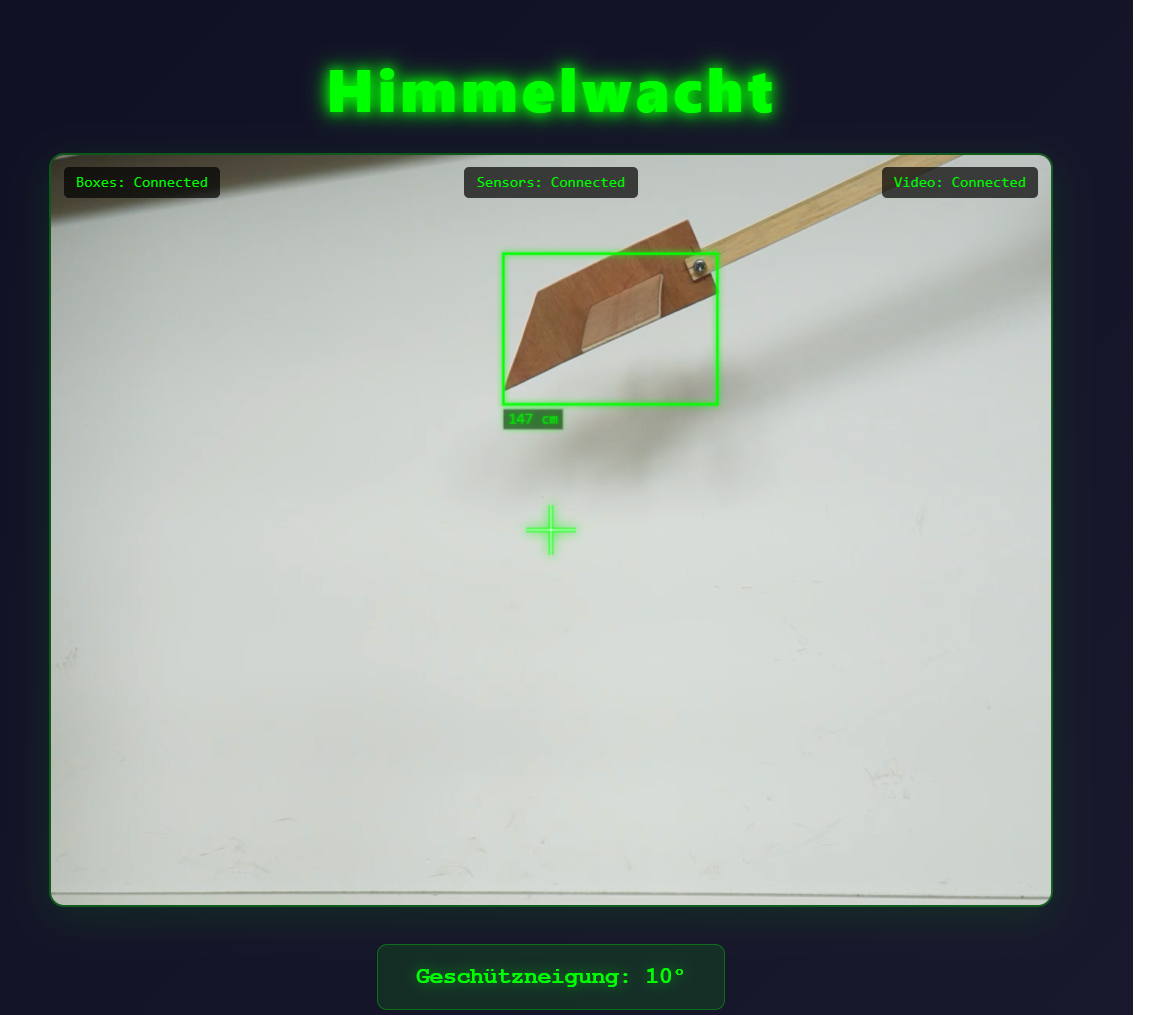
\includegraphics[width=0.8\textwidth]{images/Webserver.png}
        \caption{Webinterface zur Darstellung des Videostreams mit Bounding Boxes und Sensordaten}
        \label{fig:webserver}
    \end{center}
\end{figure}